%!TEX root = ../../thesis.tex

\section{A Neural Approach: The Stanford Attentive Reader}
\label{sec:sar}

\subsection{Preliminaries}
In the following, we outline a minimal set of elements and the key ideas which form the basis of modern neural NLP models. For more details, we refer readers to \cite{cho2015natural,goldberg2017neural}.

\subsubsection*{Word embeddings}
The first key idea is to represent words as low-dimensional (e.g., 300), real-valued vectors. Before the deep learning age, it was common to represent a word as an index into the vocabulary, which is a notational variant of using one-hot word vectors: each word is represented as a high-dimensional, sparse vector where only one entry of that word is 1 and all other entires are 0's:
\begin{eqnarray*}
\mf{v}_{\text{car}} = [0, 0, \ldots, 0, 0, 1, 0, \ldots, 0]^{\intercal} \\
\mf{v}_{\text{vehicle}} = [0, 1, \ldots, 0, 0, 0, 0, \ldots, 0]^{\intercal}
\end{eqnarray*}

The biggest problem with these sparse vectors is that they don't share any semantic similarity between words, i.e., for any pair of different words $a, b$, $\cos(\mf{v}_a, \mf{v}_b) = 0$. Low-dimensional word embeddings effectively alleviated this problem and similar words can be encoded as similar vectors in geometry space: $\cos(\mf{v}_{\text{car}}, \mf{v}_{\text{vechicle}}) < \cos(\mf{v}_{\text{car}}, \mf{v}_{\text{man}})$.

These word embeddings can be effectively learned from large unlabeled text corpora, based on the assumption that words occur in similar contexts tend to have similar meanings (a.k.a. the \ti{distributional hypothesis}). Indeed, learning word embeddings from text has a long-standing history and has been finally popularized by recent scalable algorithms and released sets of pretrained word embeddings such as \sys{word2vec}~\cite{mikolov2013distributed}, \sys{glove}~\cite{pennington2014glove} and \sys{fasttext}~\cite{bojanowski2017enriching}. They have become the mainstay of modern NLP systems.

\subsubsection*{Recurrent neural networks}
The second important idea is the use of recurrent neural networks (RNNs) to model sentences or paragraphs in NLP. \ti{Recurrent neural networks} are a class of neural networks which are suitable to handle sequences of variable length. More concretely, they apply a parameterized function recursively on a sequence $\mf{x}_1, \ldots, \mf{x}_n$:
\begin{equation}
    \mf{h}_t = f(\mf{h}_{t-1}, \mf{x}_t; \Theta)
\end{equation}
For NLP applications, we represent a sentence or a paragraph as a sequence of words where each word is transformed into a vector (usually through pre-trained word embeddings): $\mf{x} = \mf{x}_1, \mf{x}_2, \ldots, \mf{x}_n \in \R^d$ and $\mf{h}_t \in \R^h$ can be used to model the contextual information of $\mf{x}_{1:t}$.

Vanilla RNNs take the form of
\begin{equation}
    \mf{h}_t = \tanh(\mf{W}^{hh}\mf{h}_{t-1} + \mf{W}^{hx}\mf{x}_t + \mf{b}),
\end{equation}
where $\mf{W}^{hh} \in \R^{h \times h}, \mf{W}^{hx} \in \R^{h\times d}$, $\mf{b} \in \R^h$ are the parameters to be learned. To ease the optimization, many variants of RNNs have been proposed. Among them, long short-term memory networks (LSTMs)~\cite{hochreiter1997} and gated recurrent units (GRUs)~\cite{cho2014learning} are the commonly used ones. Arguably, LSTM is still the most competitive RNN variant for NLP applications today and also our default choice for the neural models that we will describe. Mathematically, LSTMs can be formulated as follows:
\begin{eqnarray}
    \mf{i}_t & = & \sigma(\mf{W}^{ih}\mf{h}_{t-1} + \mf{W}^{ix}\mf{x_t} + \mf{b}^{i}) \\
    \mf{f}_t & = & \sigma(\mf{W}^{fh}\mf{h}_{t-1} + \mf{W}^{fx}\mf{x_t} + \mf{b}^{f}) \\
    \mf{o}_t & = & \sigma(\mf{W}^{oh}\mf{h}_{t-1} + \mf{W}^{ox}\mf{x_t} + \mf{b}^{o}) \\
    \mf{g}_t & = & \tanh(\mf{W}^{gh}\mf{h}_{t-1} + \mf{W}^{gx}\mf{x_t} + \mf{b}^{g}) \\
    \mf{c}_t & = & \mf{f}_t \odot \mf{c}_{t-1} + \mf{i}_t \odot \mf{g}_t \\
    \mf{h}_t & = & \mf{o}_t \odot \tanh(\mf{c}_t),
\end{eqnarray}
where $\mf{W}^{ih}, \mf{W}^{fh}, \mf{W}^{oh}, \mf{W}^{gh} \in \R^{h \times h}$, $\mf{W}^{ix}, \mf{W}^{fx}, \mf{W}^{ox}, \mf{W}^{gx} \in \R^{h \times d}$ and $\mf{b}^{i}, \mf{b}^{f}, \mf{b}^{o}, \mf{b}^{g} \in \R^h$ are the parameters to be learned.

Finally, a useful elaboration of an RNN is a \ti{bidirectional RNN}. The idea is simple: for a sentence or a paragraph, $\mf{x} = \mf{x}_1, \ldots, \mf{x}_n$, a forward RNN is used from left to right and then another backward RNN is used from right to left:
\begin{eqnarray}
    \overrightarrow{\mf{h}}_t & = & f(\overrightarrow{\mf{h}}_{t-1}, \mf{x}_t; \overrightarrow{\Theta}), \quad t = 1, \ldots, n\\
    \overleftarrow{\mf{h}}_t & = & f(\overleftarrow{\mf{h}}_{t+1}, \mf{x}_t; \overleftarrow{\Theta}), \quad t = n, \ldots, 1
\end{eqnarray}
We define $\mf{h}_t = [\overrightarrow{\mf{h}}_t; \overleftarrow{\mf{h}}_t] \in \R^{2h}$ which takes the concatenation of the hidden vectors from the RNNs in both directions. These representations can usefully encode information from both the left context and the right context and are suitable for general-purpose trainable feature-extracting component of many NLP tasks.

\subsubsection*{Attention mechanism}
The third important component is an attention mechanism. It was first introduced in the \textit{sequence-to-sequence} (seq2seq) models \cite{sutskever2014sequence} for neural machine translation \cite{bahdanau2015neural,luong2015effective} and has later been extended to other NLP tasks.

The key idea is, if we want to predict the sentiment of a sentence, or translate a sentence of one language to the other, we usually apply recurrent neural networks to encode a single sentence (or the source sentence for machine translation): $\mf{h}_1, \mf{h}_2, \ldots, \mf{h}_n$ and use the last time step $\mf{h}_n$ to predict the sentiment label or the first word in the target language:

\begin{equation}
  P(Y = y) = \frac{\exp(\mf{W}_y\mf{h}_n)}{\sum_{y'}{\exp\left(\mf{W}_{y'}\mf{h}_n\right)}}
\end{equation}

This requires the model to be able to compress all the necessary information of a sentence into a fixed-length vector, which causes an information bottleneck in improving performance. An attention mechanism is designed to solve this problem: instead of squashing all the information into the last hidden vector, it looks at the hidden vectors at all time steps and chooses a subset of these vectors adaptively:
\begin{eqnarray}
    \alpha_i & = & \frac{\exp\left(g(\mf{h}_i, \mf{w}; \Theta_g)\right)}{\sum_{i'=1}^{n}\exp\left(g(\mf{h}_{i'}, \mf{w}; \Theta_g)\right)} \label{eq:attention} \\
    \mf{c} & = & \sum_{i=1}^{n}{\alpha_i \mf{h}_i} \label{eq:context-vector}
\end{eqnarray}

Here $\mf{w}$ can be a task-specific vector learned from the training process, or taken as the current target hidden state in machine translation and $g$ is a parameteric function which can be chosen in various ways, such as dot product, bilinear product, or one hidden layer of MLP:
\begin{eqnarray}
    g_{\text{dot}}(\mf{h}_i, \mf{w}) &=& {\mf{h}_i}^{\intercal}\mf{w} \\
    g_{\text{bilinear}}(\mf{h}_i, \mf{w}) &=& {\mf{h}_i}^\intercal\mf{W}\mf{w} \\
    g_{\text{MLP}}(\mf{h}_i, \mf{w}) &=& {\mf{v}}^\intercal\tanh(\mf{W}^h\mf{h}_i + \mf{W}^w\mf{w}) \label{eq:mlp-att}
\end{eqnarray}

Roughly, an attention mechanism computes a similarity score for each $\mf{h}_i$ and then a softmax function is applied which returns a discrete probability distribution over all the time steps. Thus $\alpha$ essentially captures which parts of the sentence are indeed relevant and $\mf{c}$ aggregates over all the time steps with a weighted sum and can be used for final prediction. We are not going into more details and interested readers are referred to \newcite{bahdanau2015neural,luong2015effective}.

Attention mechanisms have been proved widely effective in numerous applications and become an integral part of neural NLP models. Recently, \newcite{parikh2016decomposable} and \newcite{vaswani2017attention} conjectured that attention mechanisms don't have to be used in conjunction with recurrent neural networks and can be built purely based on word embeddings and feed-forward networks, while providing minimal sequence information. This class of models usually requires less parameters and is more parallelizable and scalable --- in particular, the \sys{Transformer} model proposed in \newcite{vaswani2017attention} has become a recent trend and we will discuss it more in Section~\ref{sec:alt-lstms}.

\subsection{The Model}
At this point, we are equipped with all the building blocks. How can we build effective neural models out of them for reading comprehension? What are the key ingredients? Next we introduce our model: the \sys{Stanford Attentive Reader}. Our model is inspired by the \sys{Attentive Reader} described in \newcite{hermann2015teaching} and other concurrent works, with a goal of making the model simple yet powerful. We first describe its full form for span prediction problems that we introduced in \newcite{chen2017reading} and then later we discuss its other variants.

\begin{figure}[t]
\begin{center}
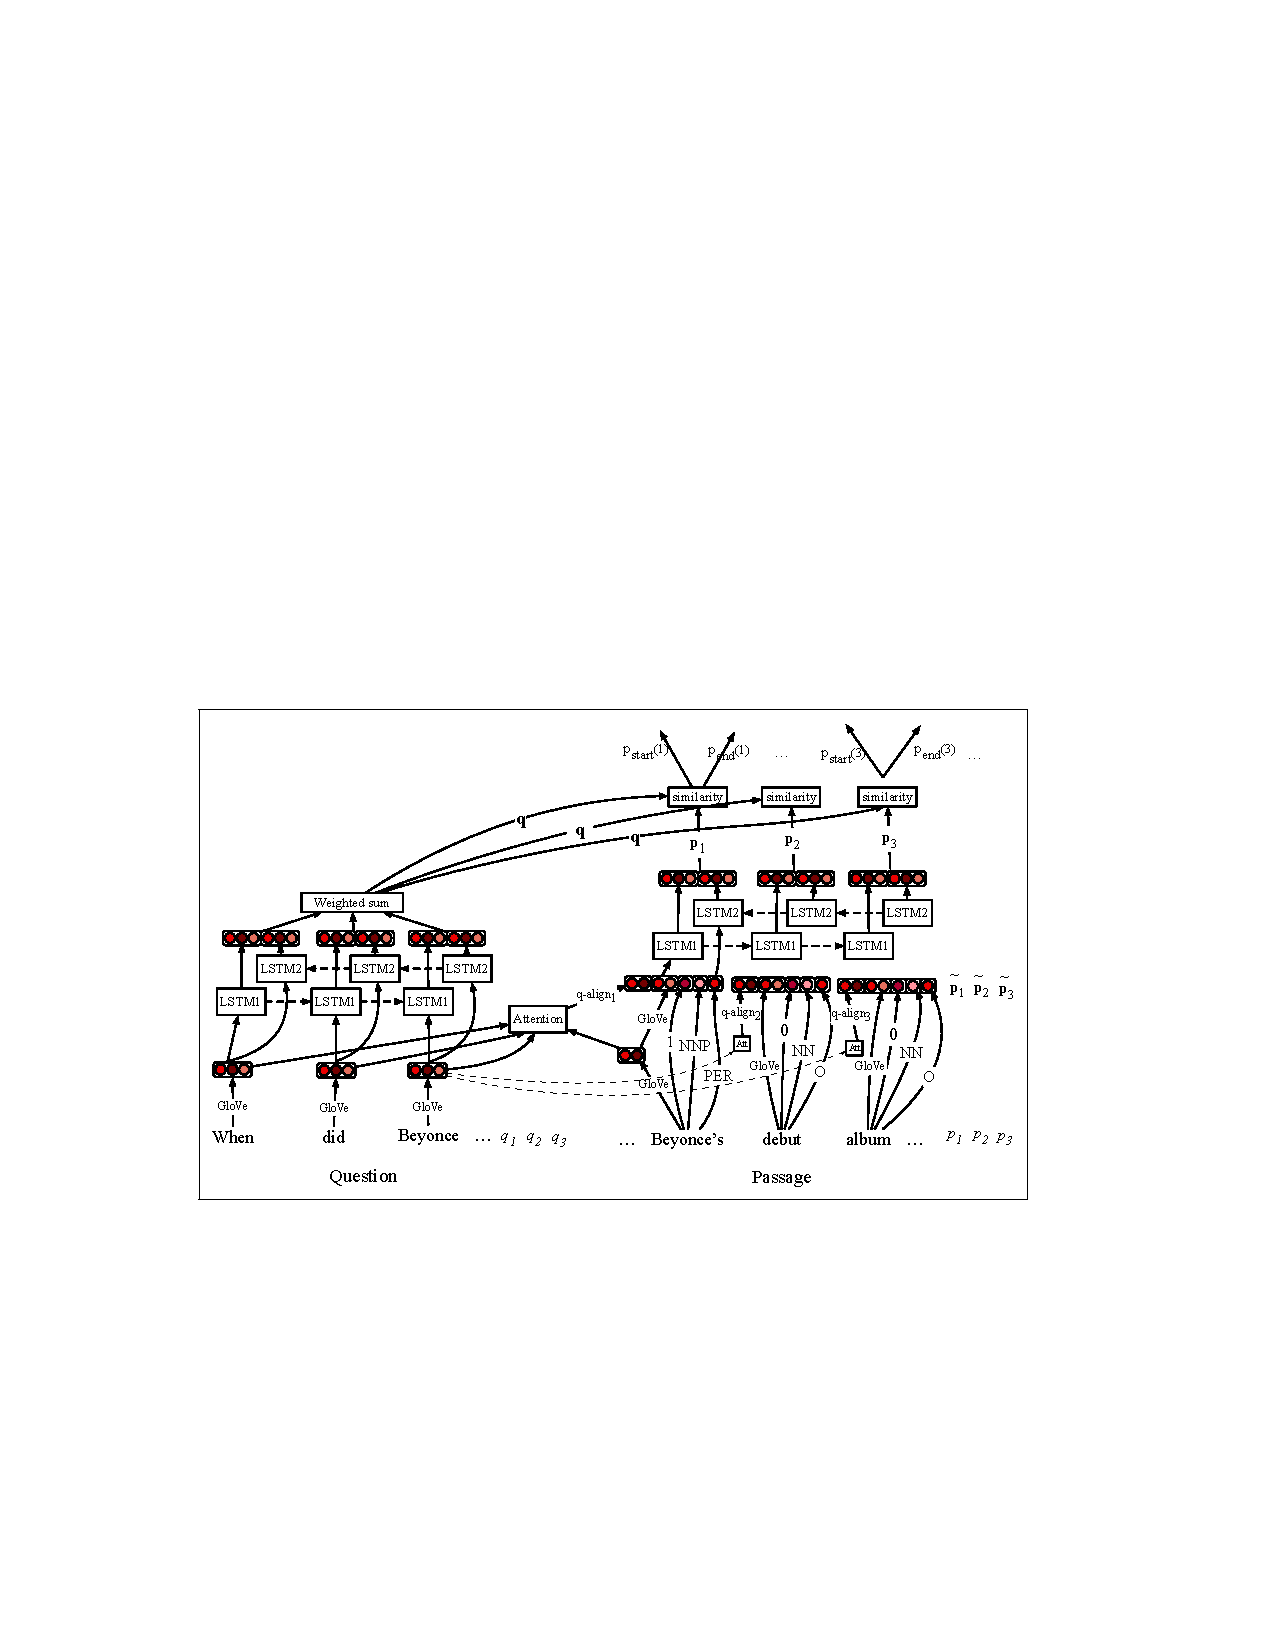
\includegraphics[height=8cm]{img/drqa_reader.pdf}
\end{center}
\longcaption{A full model of \sys{Stanford Attentive Reader}}{\label{fig:sar} A full model of \sys{Stanford Attentive Reader}. Image courtesy: \\ \href{https://web.stanford.edu/~jurafsky/slp3/23.pdf}{https://web.stanford.edu/~jurafsky/slp3/23.pdf}.}
\end{figure}

Let's first recap the setting of span-based reading comprehension problems: Given a single passage $p$ consisting of $l_p$ tokens $(p_1, p_2, \ldots, p_{l_p})$ and a question $q$ consisting of $l_q$ tokens $(q_1, q_2, \ldots, q_{l_q})$, the goal is to predict a span $(a_{\text{start}}, a_{\text{end}})$ where $1 \leq a_{\text{start}} \leq a_{\text{end}} \leq l_p$ so that the corresponding string $p_{a_{\text{start}}}, p_{a_{\text{start}} + 1}, \ldots, p_{a_{\text{end}}}$ gives the answer to the question.

The full model is illustrated in Figure~\ref{fig:sar}. At a high level, the model first builds a vector representation for the question and builds a vector representation for each token in the passage. It then computes a similarity function between the question and its passage word in context, and then uses the question-passage similarity scores to decide the starting and ending positions of the answer span. The model builds on top of the low-dimensional, pre-trained word embeddings for each word in the passage and question (with linguistic annotations optionally). All the parameters for passage/question encoding and similarity functions are optimized jointly for the final answer prediction. Let's go into further details of each component:

\subsubsection*{Question encoding}
\label{sec:question-encoding}
The question encoding is relatively simple: we first map each question word $q_i$ into its word embedding $\mf{E}(q_i) \in \R^d$ and then we apply a bi-directional LSTM on top of them and finally obtain:
\begin{equation}
    \mf{q}_{1}, \mf{q}_2, \ldots, \mf{q}_{l_q} = \text{BiLSTM}(\mf{E}(q_1), \mf{E}(q_2), \ldots, \mf{E}(q_{l_q}); \Theta^{(q)}) \in \R^{h}
\end{equation}

We then aggregate these hidden units into one single vector through an attention layer:
\begin{eqnarray}
    b_j & = & \frac{\exp({\mf{w}^{q}}^\intercal \mf{q}_j)}{\sum_{j'}{\exp({\mf{w}^{q}}^\intercal \mf{q}_{j'})}} \\
    \mf{q} & = & \sum_j{b_j \mf{q}_j}
\end{eqnarray}
$b_j$ measures the importance of each question word and $\mf{w}^{q} \in \R^h$ is a weight vector to be learned. Therefore, $\mf{q} \in \R^h$ is the final vector representation for the question. Indeed, it was simpler (and also common) to represent $\mf{q}$ as the concatenation of the last hidden vector from the LSTMs in both directions. However, based on the empirical performance, we find that adding this attention layer helps consistently as it adds more weight to the more relevant question words.

\subsubsection*{Passage encoding}
Passage encoding is similar, as we also first form an input representation $\tilde{\mf{p}}_i \in \R^{\tilde{d}}$ for each word in the passage and pass them through another bidirectional LSTM:
\begin{equation}
  \label{eq:passage-lstm}
    \mf{p}_{1}, \mf{p}_2, \ldots, \mf{p}_{l_p} = \text{BiLSTM}\left(\tilde{\mf{p}}_1, \tilde{\mf{p}}_2, \ldots, \tilde{\mf{p}}_{l_p}; \Theta^{(p)}\right) \in \R^{h}
\end{equation}

The input representation $\tilde{\mf{p}}_i$ can be divided into two categories: one is to encode \ti{the properties of each word itself}, and the other is to encode \ti{its relevance with respect to the question}.

For the first category, in addition to word embedding $f_{emb}(p_i) = \mf{E}(p_i) \in \R^d$, we also add some manual features which reflect the properties of word $p_i$ in its context, including its part-of-speech (POS) and named entity recognition (NER) tags and its (normalized) term frequency (TF): $f_{token}(p_i) = \left(\text{POS}(p_i), \text{NER}(p_i), \text{TF}(p_i)\right)$. For POS and NER tags, we run off-the-shelf tools and convert it into a one-hot representation as the set of tags is small. The TF feature is real-valued number which measures how many times the word appears in the passage divided by the total number of words.

For the second category, we consider two types of representations:
\begin{itemize}
  \item
  \tf{Exact match}: $f_{exact\_match}(p_i) = \mathbb{I}(p_i \in q) \in \R$. In practice, we use three simple binary features, indicating whether $p_i$ can be exactly matched to one question word in $q$, either in its original, lowercase or lemma form.
  \item
  \tf{Aligned question embeddings}: The exact match features encode the hard alignment between question words and passage words. Aligned question embeddings aim to encode a soft notion of alignment between words in the word embedding space, so that similar (but non-identical) words, e.g., \textit{car} and \textit{vehicle}, can be well aligned. Concretely, we use
  \begin{equation}
      \label{eq:aligned_question}
    f_{align}(p_i) = \sum_j{a_{i, j} \mf{E}(q_j)}
  \end{equation}
  where $a_{i, j}$ are the attention weights which capture the similarity between $p_i$ and each question words $q_j$ and $\mf{E}(q_j) \in \R^d$ is the word embedding for each question word. $a_{i, j}$ is computed by the dot product between nonlinear mappings of word embeddings:
  \begin{equation}
    \label{eq:aligned_question_attention}
    a_{i, j} = \frac{\exp\left(\text{MLP}(\mf{E}(p_i))^{\intercal} \text{MLP}(\mf{E}(q_{j}))\right)}{\sum_{j'}{\exp\left(\text{MLP}(\mf{E}(p_i)) ^{\intercal} \text{MLP}(\mf{E}(q_{j'}))\right)}},
  \end{equation} and $\text{MLP}(\mf{x}) = \max(0, \mf{W}_{\text{MLP}}\mf{x} + \mf{b}_{\text{MLP}})$ is a single dense layer with ReLU nonlinearity, where $\mf{W}_{\text{MLP}} \in \R^{d \times d}$ and $\mf{b}_{\text{MLP}} \in \R^d$.
\end{itemize}
Finally, we simply concatenate the four components and form the input representation:
\begin{equation}
    \tilde{\mf{p}_i} = (f_{emb}(p_i), f_{token}(p_i), f_{exact\_match}(p_i), f_{align}(p_i)) \in \R^{\tilde{d}}
\end{equation}

\subsubsection*{Answer prediction}
We have vector representations for both the passage $\mf{p}_1, \mf{p}_2, \ldots, \mf{p}_{l_p} \in \R^h$ and the question $\mf{q} \in \R^h$ and the goal is to predict the span that is most likely the correct answer. We employ the idea of attention mechanism again and train two separate classifiers, one is to predict the start position of the span while the other is to predict the end position. More specifically, we use a bilinear product to capture the similarity between $\mf{p}_i$ and $\mf{q}$:
\begin{eqnarray}
P^{(\text{start})}(i) & = & \frac{\exp\left(\mf{p}_i \mf{W}^{(\text{start})} \mf{q}\right)}{\sum_{i'}\exp\left(\mf{p}_{i'} \mf{W}^{(\text{start})} \mf{q}\right)} \\
P^{(\text{end})}(i) & = & \frac{\exp\left(\mf{p}_i \mf{W}^{(\text{end})} \mf{q}\right)}{\sum_{i'}\exp\left(\mf{p}_{i'} \mf{W}^{(\text{end})} \mf{q}\right)},
\end{eqnarray}
where $\mf{W}^{(\text{start})}, \mf{W}^{(\text{end})} \in \R^{h \times h}$ are additional parameters to be learned. This is slightly different from the formulation of attention as we don't need to take the weighted sum of all the vector representations. Instead, we use the normalized weights to make direct predictions. We use bilinear products because we find them to work well empirically.

\subsubsection*{Training and inference}
The final training objective is to minimize the cross-entropy loss:
\begin{equation}
    \mathcal{L} = - \sum \log{P^{(\text{start})}(a_{\text{start}})} - \sum \log{P^{(\text{end})}(a_{\text{end}})},
\end{equation}
and all the parameters $\Theta = \Theta^{(p)}, \Theta^{(q)}, \mf{w}^{(q)}, \mf{W}_{\text{MLP}}, \mf{b}_{\text{MLP}}, \mf{W}^{(\text{start})}, \mf{W}^{(\text{end})}$ are optimized jointly with stochastic gradient methods.\footnote{We exclude word embeddings here but it is also common to treat all or a subset of the word embeddings as parameters and fine-tune them during training.}

During inference, we choose the span $p_i, \ldots, p_{i'}$ such that $i \leq i' \leq i + max\_len$ and $P^{(\text{start})}(i) \times P^{(\text{end})}(i')$ is maximized. $max\_len$ is a pre-defined constant (e.g., 15) which controls the maximum length of the answer.

\subsection{Extensions}
In the following, we give a few variants of the \sys{Stanford Attentive Reader} for other types of reading comprehension problems.
All these models follow the same process of passage encoding and question encoding as described above, hence we have $\mf{p}_1, \mf{p}_2, \ldots, \mf{p}_{l_p} \in \R^h$ and $\mf{q} \in \R^h$. We only discuss the answer prediction component and training objectives.

\paragraph{\tf{Cloze style.}} Similarly, we can compute an attention function using a bilinear product of the question over all the words in the passage, and then compute an output vector $\mf{o}$ which takes a weighted sum of all the paragraph representations:
\begin{eqnarray}
    \alpha_i & = & \frac{\exp\left(\mf{p}_i \mf{W} \mf{q}\right)}{\sum_{i'}\exp\left(\mf{p}_{i'} \mf{W} \mf{q}\right)} \\
    \mf{o} & = & \sum_{i}{\alpha_i \mf{p}_i}   \label{eqn:output_vector}
\end{eqnarray}
The output vector $\mf{o}$ can be used to predict the missing word or entity:
\begin{equation}
    P(Y = e \mid p, q) = \frac{\exp(\mf{W}^{(a)}_e \mf{o})}{\sum_{e' \in \mathcal{E}}\exp\left(\mf{W}^{(a)}_{e'} \mf{o}\right)},
\end{equation}
where $\mathcal{E}$ denotes the candidate set of entities or words. It is straightforward to adopt a negative log-likelihood objective for training and choose $e \in \mathcal{E}$ which maximizes $\mf{W}^{(a)}_{e} \mf{o}$ during prediction. This model has been studied in our earlier paper \cite{chen2016thorough} for the \sys{CNN/Daily Mail} dataset and \cite{onishi2016did} for the \sys{Who-Did-What} dataset.

\paragraph{\tf{Multiple choice.}} In this setting, $k$ hypothesized answers are given $\mathcal{A} = \{a_1, \ldots, a_k\}$ and we can encode each of them into a vector $\mf{a}_i$ by applying a third BiLSTM, similar to our question encoding step. We can then compute the output vector $\mf{o}$ as in Equation~\ref{eqn:output_vector} and compare it with each hypothesized answer vector $\mf{a}_i$ through another similarity function using a bilinear product:
\begin{equation}
    P(Y = i \mid p, q) = \frac{\exp(\mf{a}_i \mf{W}^{(a)} \mf{o})}{\sum_{i'=1, \ldots, k}\exp\left(\mf{a}_{i'}\mf{W}^{(a)} \mf{o}\right)}
\end{equation}
The cross-entroy loss is also used for training. This model has been studied in \newcite{lai2017race} for the \sys{RACE} dataset.

\paragraph{\tf{Free-form answer.}} For this type of problems, the answer isn't restricted to a single entity or a span in the passage and can take any sequence of words and the most common solution is to incorporate an LSTM sequence decoder into the current framework. In more detail, assume the answer string is $a = (a_1, a_2, \ldots, a_{l_a})$ and a special ``end-of-sequence'' token $\left<eos\right>$ is added to the end of each answer. We can compute the output vector $\mf{o}$ again as in Equation~\ref{eqn:output_vector}. and the decoder generates a word at a time and hence the conditional probability can be decomposed as:
\begin{equation}
    P(a \mid p, q) =  P(a \mid \mf{o}) = \prod_{j = 1}^{l_a}P(a_j \mid a_{<j}, \mf{o})
\end{equation}

$P(a_j \mid a_{<j}, \mf{o})$ is parameterized as an LSTM which takes $\mf{o}$ as the initial hidden vector, and $a_j$ is predicted based on the hidden vector $\mf{h}_j$ for the full vocabulary $\mathcal{V} \cup \{\left<eos\right>\}$. The training objective is
\begin{equation}
\mathcal{L} = -\log{P(a \mid p, q)} = -\log\sum_{j = 1}^{l_a}P(a_j \mid a_{<j}, \mf{o})
\end{equation}
For prediction, one word is predicted at a time which maximizes $P(a_j \mid a_{<j}, \mf{o})$ and then fed into the next time step, until the token $\left<eos\right>$ is predicted. We are not going to elaborate more on it as they are standard components in sequence-to-sequence models \cite{sutskever2014sequence}.

This class of models has been studied on the \sys{MS MARCO}~\cite{nguyen2016ms} and the \sys{NarrativeQA}~\cite{kovcisky2018narrativeqa} datasets. However, as the free-form answer reading comprehension problems are more complex and more difficult to evaluate, we think that these methods haven't been fully explored yet, compared to other types of problems. Lastly, we believe that a \textit{copy mechanism} proposed for summarization tasks  \cite{gu2016incorporating,see2017get}, which allows the decoder to choose either to copy a word from the source text or to generate a word from the vocabulary, would be highly useful for reading comprehension tasks as well, as answer words are still likely to appear in the paragraph or question. We will discuss one model with a copy mechanism in Section~\ref{sec:coqa-models}.
